\documentclass[conference]{IEEEtran}
\IEEEoverridecommandlockouts
% The preceding line is only needed to identify funding in the first footnote. If that is unneeded, please comment it out.
\usepackage{cite}
\usepackage{amsmath,amssymb,amsfonts}
\usepackage{algorithmic}
\usepackage{graphicx}
\usepackage{textcomp}
\usepackage{xcolor}
\usepackage[T1]{fontenc}
\usepackage[utf8]{inputenc}
\bibliographystyle{IEEEtran}
\def\BibTeX{{\rm B\kern-.05em{\sc i\kern-.025em b}\kern-.08em
    T\kern-.1667em\lower.7ex\hbox{E}\kern-.125emX}}
\begin{document}

\title{Automated, Interpretable Quality Control for One-Photon Calcium Imaging:\\ A Machine-Learning Neuron Screening System\\

\thanks{This work was supported by the Non-commercial Foundation for the Advancement of Science and Education ``INTELLECT''. N.P. acknowledges the support of the Brain program of the IDEAS Research Center.}
}

\author{\IEEEauthorblockN{Nikita Pospelov}
\IEEEauthorblockA{\textit{Laboratory of Neuronal Intelligence} \\ \textit{Institute for Advanced Brain Studies} \\
\textit{Lomonosov Moscow State University}\\
Moscow, Russia \\
pospelov.na14@physics.msu.ru}
\and
\IEEEauthorblockN{Olga Rogozhnikova}
\IEEEauthorblockA{\textit{Laboratory of Neuronal Intelligence} \\
\textit{Institute for Advanced Brain Studies} \\
\textit{Lomonosov Moscow State University}\\
Moscow, Russia \\
osrogozhnikova@gmail.com}
\and
\IEEEauthorblockN{Viktor Plyusnin}
\IEEEauthorblockA{\textit{Laboratory of Neuronal Intelligence} \\
\textit{Institute for Advanced Brain Studies} \\
\textit{Lomonosov Moscow State University}\\
Moscow, Russia \\
witkax@mail.ru}
\and
\IEEEauthorblockN{Anna Ivanova}
\IEEEauthorblockA{\textit{Laboratory of Neuronal Intelligence} \\
\textit{Institute for Advanced Brain Studies} \\
\textit{Lomonosov Moscow State University}\\
Moscow, Russia \\
anivis33@gmail.com}
\and
\IEEEauthorblockN{Ksenia Toropova}
\IEEEauthorblockA{\textit{Laboratory of Neuronal Intelligence} \\
\textit{Institute for Advanced Brain Studies} \\
\textit{Lomonosov Moscow State University}\\
Moscow, Russia \\
xen.alexander@gmail.com}
\and
\IEEEauthorblockN{Olga Ivashkina}
\IEEEauthorblockA{\textit{Laboratory of Neuronal Intelligence} \\
\textit{Institute for Advanced Brain Studies} \\
\textit{Lomonosov Moscow State University}\\
Moscow, Russia \\
oivashkina@gmail.com}
\and
\IEEEauthorblockN{Konstantin Anokhin}
\IEEEauthorblockA{\textit{Laboratory of Neuronal Intelligence} \\
\textit{Institute for Advanced Brain Studies} \\
\textit{Lomonosov Moscow State University}\\
Moscow, Russia \\
k.anokhin@gmail.com}
}
\maketitle

\begin{abstract}
Manual curation of candidate neurons is a persistent bottleneck in one-photon calcium imaging: automated component extraction deliberately over-segments to preserve sensitivity, leaving experts to inspect hundreds to thousands of candidates per session by hand. We present an automated screening system that reproduces expert-level decisions while remaining fully transparent. Each candidate is described by 35 interpretable features spanning spatial morphology, trace statistics, calcium-event properties, reconstruction quality, and extractor-provided metrics. A cascading kinetics-estimation procedure recovers event-based features for neurons on which standard event detection fails, raising coverage from 42\% to 80\% of candidates. Classification uses an Explainable Boosting Machine optimized for an asymmetric $F_\beta$ objective ($\beta=0.577$) that penalizes false positives three times more heavily than false negatives. Validated by session-stratified cross-validation on 92{,}242 neurons from 187 recording sessions across four experimental paradigms, the system attains 97.6\% precision and 93.3\% recall (AUC 0.978), reducing curation from hours to minutes while providing a per-feature audit trail for every decision.
\end{abstract}

\begin{IEEEkeywords}
calcium imaging, quality control, interpretable machine learning, explainable boosting machine, neuron curation, active learning
\end{IEEEkeywords}

\section{Introduction}

One-photon calcium imaging with miniaturized microscopes (miniscopes) records the activity of large neuronal populations in freely behaving animals. Extracting single-neuron signals from this data relies on automated decomposition algorithms such as CNMF-E \cite{Zhou2018}, implemented in the CaImAn suite \cite{Giovannucci2019}. By design these algorithms prioritize sensitivity over specificity: they over-segment the field of view so that no genuine neuron is missed, accepting that many false candidates -- arising from motion artifacts, neuropil contamination, imaging aberrations, and edge effects -- will be produced alongside real cells.

The standard workflow therefore ends with a manual step. An expert inspects every candidate, weighing its spatial footprint, temporal activity, and quality metrics, and labels it a neuron or an artifact. For a typical session of 500--1500 candidates this requires one to three hours of focused attention. Beyond the time cost, manual curation is subjectively inconsistent: annotators disagree on borderline cases, and the criteria that distinguish a ``real'' neuron remain largely implicit, hard to articulate, standardize, or transfer.

We address this final bottleneck with an automated, interpretable screening system. Our contribution is fourfold: (i) a 35-dimensional interpretable feature space that makes implicit curation criteria explicit; (ii) a cascading kinetics-estimation procedure that recovers informative event-based features for difficult neurons; (iii) a glass-box Explainable Boosting Machine (EBM) classifier trained against an asymmetric-cost objective; and (iv) a validation at scale -- 92{,}242 expert-labeled neurons from 187 sessions -- establishing expert-level accuracy with a complete decision audit trail.

\section{Methods}

\subsection{Animals, imaging, and preprocessing}

Experiments were performed on male and female C57Bl/6 mice aged 3--5 months. Activity of CA1 neurons was recorded with a miniature microscope (UCLA Miniscope V4.4, OpenEphys). Animals underwent stereotaxic surgery in which viral particles carrying the gene of the fluorescent calcium sensor GCaMP6s were injected into hippocampal area CA1, a GRIN lens (1~mm) was implanted, and a baseplate for the miniscope was fixed. Animal behavior was captured with a video camera (FLIR Chameleon 3), and the two data streams were synchronized in the Bonsai environment \cite{lopes2015bonsai}. All animal-care procedures and experimental protocols were approved by the Animal Care Committee of Lomonosov Moscow State University (application No.~159-a, approved by the Bioethics Commission, meeting No.~154-d of 17.08.2023) and complied with Order No.~267 of the Ministry of Health of the Russian Federation and the US NIH Guide for the Care and Use of Laboratory Animals.

Calcium-activity analysis was performed with the authors' BEARMIND package (\texttt{https://github.com/iabs-neuro/bearmind}), built on CaImAn \cite{Giovannucci2019}. After visual inspection and spatial cropping, video was preprocessed in a streaming fashion with NoRMCorre motion correction \cite{Pnevmatikakis2017} and CNMF-E component extraction \cite{Zhou2018}. Fluorescence traces were normalized as $dF/F$, and spatial footprints were registered across sessions with CellReg \cite{Sheintuch2017}. The resulting candidate components -- the input to our screening system -- comprise the labeled dataset of \textbf{92{,}242 neurons from 187 sessions} across four experimental paradigms (LNOF: 49{,}767; NOF: 30{,}398; RFC: 7{,}505; FOF: 4{,}572), each candidate manually labeled as a genuine neuron (81.1\%) or an artifact (18.9\%) by expert curators.

\subsection{Interpretable feature space}

No single metric separates neurons from artifacts: real cells vary widely in size, intensity, and activity, while artifacts can mimic neuronal footprints. We therefore characterize each candidate with 35 features in five complementary groups:

\begin{itemize}
\item \emph{Spatial/morphological} (11): area, circularity, convexity, aspect ratio, eccentricity, compactness, distance to image edge, and neighborhood relations -- flagging implausible shapes and boundary artifacts.
\item \emph{Temporal/trace} (9): skewness, kurtosis, baseline drift, noise level, bimodality, and the Hurst exponent of the $dF/F$ trace -- capturing the ``spiky'' signature of genuine calcium dynamics.
\item \emph{Event-based} (8): rate, fit quality, signal-to-noise, rise/decay times, and amplitude variability of detected calcium transients, obtained with the DRIADA event detector \cite{Sych2019}.
\item \emph{Reconstruction} (4): $R^2$, NMAE, NRMSE, and residual SNR of a single-compartment calcium-dynamics fit.
\item \emph{Extractor-provided} (2): CaImAn SNR and spatial-correlation score, plus two metadata features tracking the characterization process.
\end{itemize}

\subsection{Cascading kinetics estimation}

Event-based features are among the most discriminative, but standard event detection fails on 40--60\% of candidates (low SNR, sparse firing, non-standard kinetics, or baseline nonstationarity), leaving eight features undefined. Discarding these candidates would remove many genuine but hard-to-characterize neurons -- precisely the cases where automation is most valuable.

We instead apply a five-tier fallback cascade that attempts progressively more permissive characterizations: (1) wavelet detection with strict criteria; (2) wavelet detection with relaxed thresholds (min.\ 3 events, fit $R^2\geq0.6$); (3) an alternative threshold-based detector with standard criteria; (4) the threshold detector with relaxed criteria; (5) physically plausible default kinetics when all detectors fail. The first successful tier is recorded as an explicit feature, so the classifier can weight event-based information by its reliability. The cascade lifts the fraction of candidates with genuine event features from 42\% (single attempt) to 80\%, and the system never fails outright: spatial, trace, and reconstruction features remain available even at tier~5 (graceful degradation).

\subsection{Classifier and decision objective}

We classify candidates with an Explainable Boosting Machine (EBM) \cite{Lou2013,Nori2019}, a generalized additive model that expresses the decision as a sum of per-feature shape functions plus a small number of learned pairwise interactions. Unlike black-box ensembles, every prediction decomposes exactly into the contribution of each feature, yielding a complete audit trail (e.g.\ $+0.32$ from trace skewness, $-0.15$ from area) while matching the accuracy of random forests and gradient boosting. The production model uses 35 features and 20 automatically selected interactions; hyperparameters were chosen by stratified cross-validation over 128 configurations.

Classification errors are asymmetric: a false positive (an artifact kept as a neuron) can corrupt population statistics, whereas a false negative merely costs statistical power. We therefore optimize the $F_\beta$ score
\begin{equation}
F_\beta = (1+\beta^2)\,\frac{\mathrm{precision}\cdot\mathrm{recall}}{\beta^2\,\mathrm{precision}+\mathrm{recall}},
\label{eq:fbeta}
\end{equation}
with $\beta=\sqrt{1/3}\approx0.577$ \cite{vanRijsbergen1979}, penalizing false positives three times more heavily than false negatives. The system supports three deployment modes -- transparent rule-based filtering for clear-cut cases, EBM scoring with a tunable threshold for borderline cases, and a hybrid that applies rules first and the EBM to the remainder -- letting users trade precision against recall to match each experimental context.

\section{Results}

\subsection{Classification performance}

We evaluated the system by cross-validation stratified \emph{by recording session}, so that neurons from one session never appear in both training and test folds; this prevents the model from exploiting session-specific imaging conditions and tests genuine generalization. The production model (v9) attains, across folds (mean\,$\pm$\,s.d.):

\begin{center}
\begin{tabular}{lc}
\hline
Metric & Value \\
\hline
$F_\beta$ ($\beta=0.577$) & $0.965 \pm 0.004$ \\
Precision & $0.976 \pm 0.003$ \\
Recall & $0.933 \pm 0.007$ \\
AUC-ROC & $0.978 \pm 0.005$ \\
\hline
\end{tabular}
\end{center}

A precision of 97.6\% means only 2.4\% of accepted candidates are artifacts; a recall of 93.3\% means 6.7\% of genuine neurons are missed -- a trade-off deliberately favoring precision. The low cross-session variance confirms stable performance across imaging conditions and paradigms.

\subsection{Which features matter}

Feature-importance analysis (Fig.~\ref{fig:importance}) shows that temporal trace statistics carry the strongest discriminative power: trace skewness and kurtosis rank first and second. This validates what annotators report anecdotally -- they look for the characteristic spiky, heavy-tailed appearance of genuine calcium traces. Notably, the extractor's own SNR ranks near the bottom, whereas event-based SNR computed from detected transients ranks among the top features, showing that temporal structure is far more informative than raw amplitude.

\begin{figure}[t]
\centering
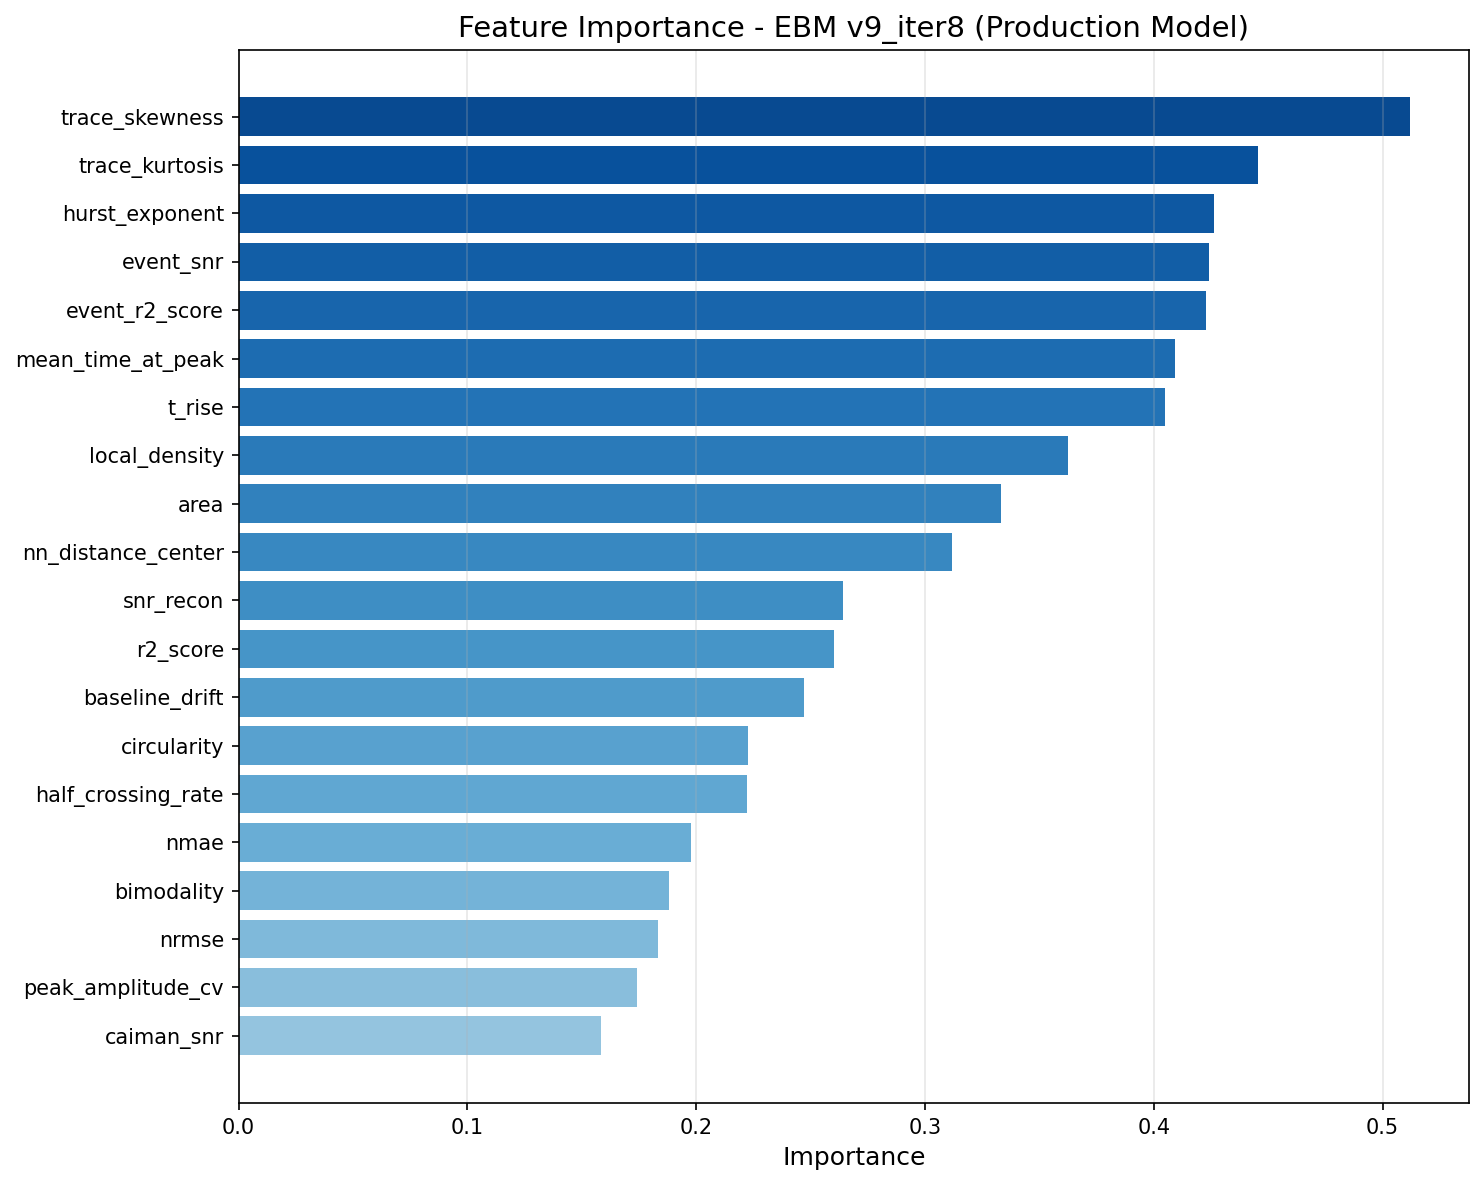
\includegraphics[width=\columnwidth]{figs/figure1_feature_importance.png}
\caption{Feature importance for the production EBM classifier. Temporal trace statistics (skewness, kurtosis) dominate, followed by the Hurst exponent and event-based metrics. The extractor-provided CaImAn SNR ranks lowest, underscoring the value of analyzing temporal structure over simple amplitude.}
\label{fig:importance}
\end{figure}

\subsection{Tuning the operating point}

Because the EBM emits a calibrated score, a single threshold tunes the precision/recall balance. Fig.~\ref{fig:threshold} shows the $F_\beta$ score and the false-positive/false-negative trade-off as the threshold varies. Total error is minimized near a threshold of 0.72--0.75; higher thresholds (0.7--0.8) maximize precision for publication-grade datasets, while lower thresholds (0.3--0.4) maximize recall for exploratory screening.

\begin{figure}[t]
\centering
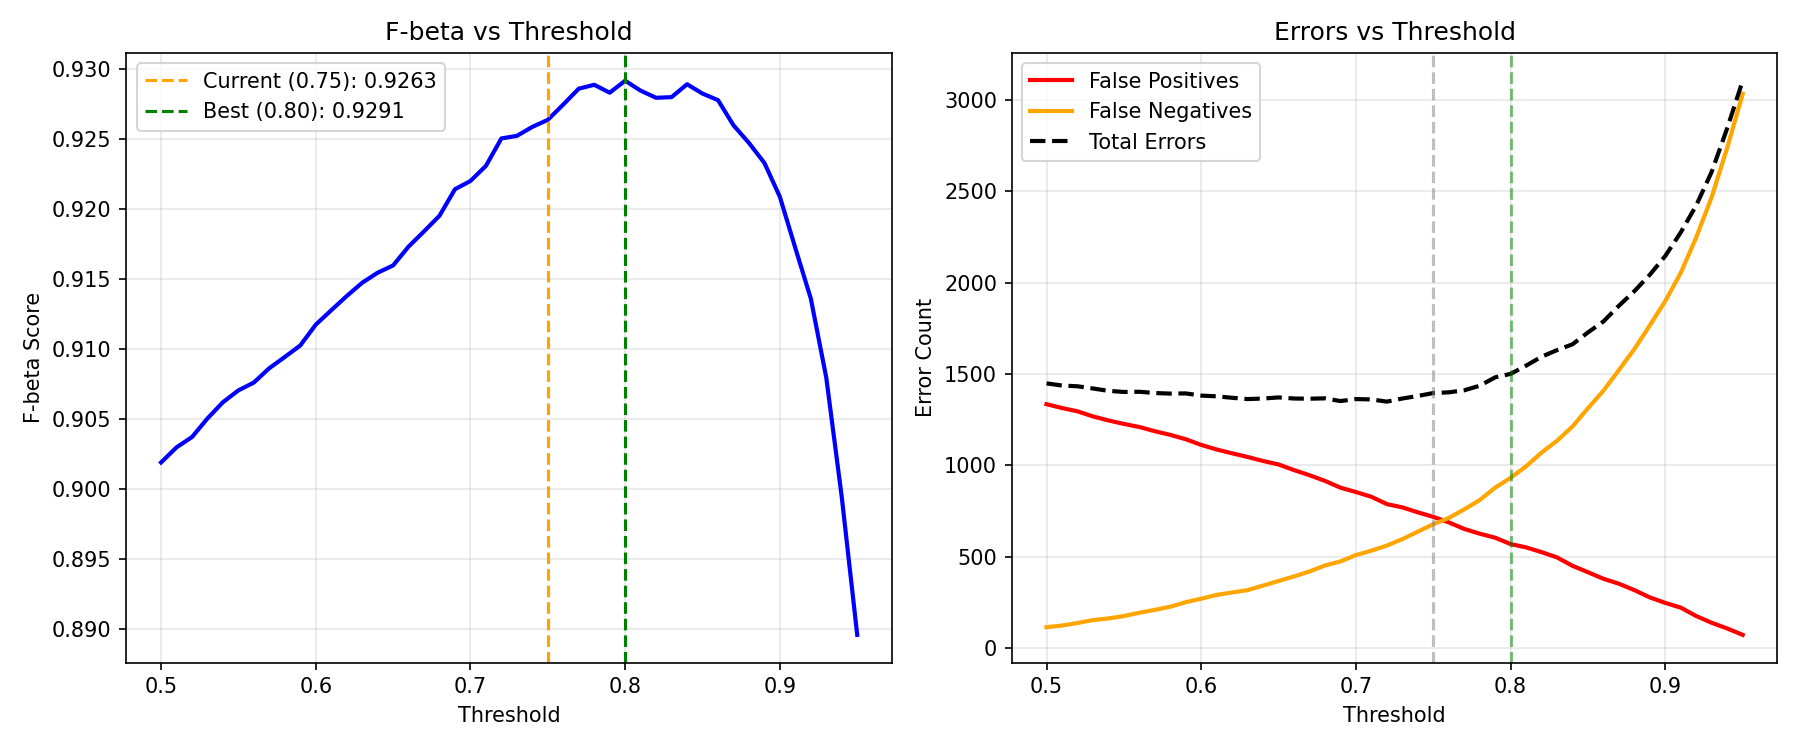
\includegraphics[width=\columnwidth]{figs/figure2_threshold_analysis.png}
\caption{Threshold optimization. Left: $F_\beta$ ($\beta=0.577$) versus decision threshold, with the operating and optimal points marked. Right: false positives (red) and false negatives (orange) versus threshold; total error (dashed) is minimized around 0.72--0.75.}
\label{fig:threshold}
\end{figure}

\subsection{Practical impact}

Manual curation of a 1000-candidate session takes one to two hours; the automated system -- feature extraction, classification, and report generation -- processes the same session in two to three minutes, a 30--40$\times$ speedup that enables same-day analysis of newly acquired data. Because identical criteria are applied to every candidate, results are fully reproducible, and the per-feature audit trail lets researchers see exactly why each decision was made.

\section{Discussion and Conclusion}

We have presented an automated quality-control system that closes the last manual step in calcium-imaging preprocessing. Three design principles -- comprehensive feature engineering, graceful degradation, and transparency -- let it reach expert-level accuracy (97.6\% precision, 93.3\% recall) without becoming a black box.

Interpretability is not merely cosmetic: it enables an active-learning loop. When a researcher reviews a classification, the audit trail shows which features drove it; a corrected label becomes a training example for the next model iteration, so that implicit expert knowledge is progressively captured and scaled. Across eight iterations of the current model version, such corrections yielded measurable gains in precision and AUC on initially problematic cases.

The system has limitations. It was trained on one-photon miniscope recordings of cortical and hippocampal neurons expressing GCaMP indicators; transfer to other modalities (two-photon, voltage, light-sheet) or markedly different cell types may require retraining. Entirely silent neurons remain inherently ambiguous, and roughly 20\% of candidates still rely on default kinetics. Natural extensions include tighter integration with upstream extractors, real-time quality assessment during acquisition, and principled session-specific calibration.

More broadly, this work shows that interpretable machine learning can match expert judgment in a scientific decision task while remaining auditable. By making implicit curation criteria explicit and enabling continuous refinement through feedback, the system scales and preserves human expertise rather than hiding it behind opaque automation, and -- combined with CNMF-E extraction -- enables a fully automated pipeline from raw miniscope video to verified neural populations.

% \section*{Acknowledgment}
% Optional: add personal acknowledgments here if desired.

\bibliography{references}

\end{document}
